\documentclass[{../../master}]{subfiles}
\graphicspath{{../..}}  % 個別コンパイル時の画像パスを解決する

\begin{document}

\section{\textsf{lidar\_link}の作成と追加}
\label{sec:add_lidar_link}

RPLiDARのリンクをロボットモデルに追加します.
ロボットの部品の中でも,センサは特に座標変換が重要になるコンポーネントです.
センサのデータシートやマニュアルをよく読んで,適切な座標変換ができるようにしましょう.

\subsection{RPLiDAR A2の光学窓}

RPLiDAR A2M6のデータシートを見ると,RPLiDAR A2の光学窓は図\ref{fig:rplidar_a2_optical_window}のようになっており,センサの底面から\SI{30.8}{mm}の高さに位置していることがわかります.
URDFを記述するときは,\textsf{lidar\_link}のリンク座標系の原点がこの位置になるようにしなければなりません.

\begin{figure}[ht]
  \centering
  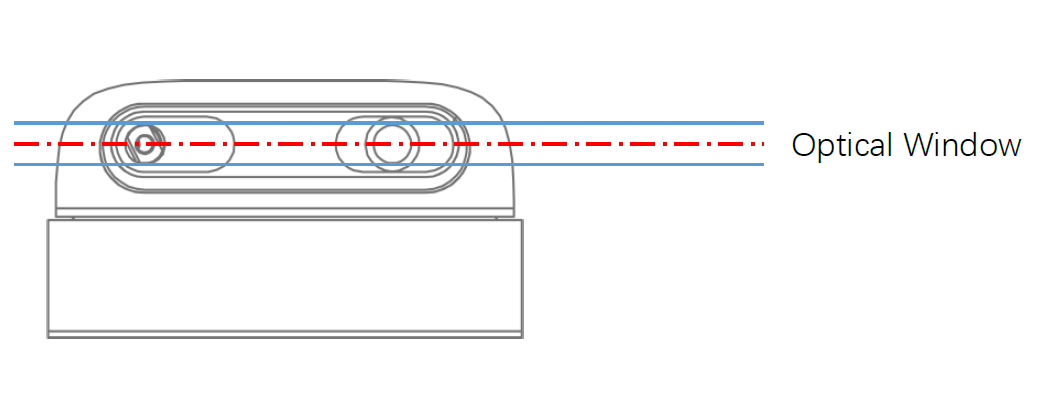
\includegraphics[width=100truemm]{images/rplidar_a2_optical_window.png}
  \label{fig:rplidar_a2_optical_window}
  \caption{RPLiDAR A2 Optical Window}
\end{figure}

\subsection{RPLiDAR A2の座標系}

RPLiDAR A2は少々特殊な座標系を持っており,その向きは図\ref{fig:rplidar_a2_coordinate_system}に示す通りになっています.

\begin{figure}[ht]
  \centering
  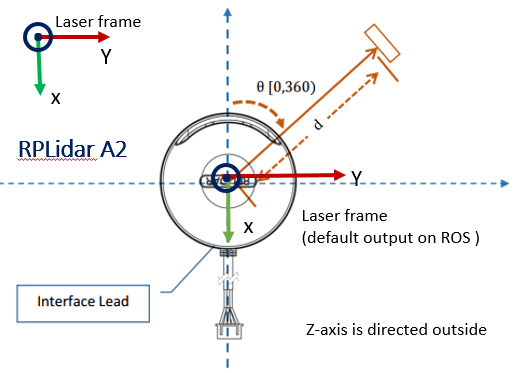
\includegraphics[width=100truemm]{images/rplidar_a2_coordinate_system.png}
  \label{fig:rplidar_a2_coordinate_system}
  \caption{Coordinate System of RPLiDAR A2}
\end{figure}

図を見るとわかるのですが,ROS REP:103で推奨されている座標系と一致していません(Z軸周りに180度回転させた向きになっている).
そのため,モデルの見た目とセンサデータの座標変換とを両立させるために,ジョイントの向きを図\ref{fig:rplidar_a2_coordinate_system}の通りにし,モデルの見た目を180度回転させる,という処理が必要になります.

\subsection{STLファイルの作成}

STLファイルの出力座標系は図\ref{fig:lidar_link_coordinate}のようにします.
座標系の原点はセンサ底面から\SI{30.8}{mm}の高さに位置しています.

\begin{figure}[ht]
  \centering
  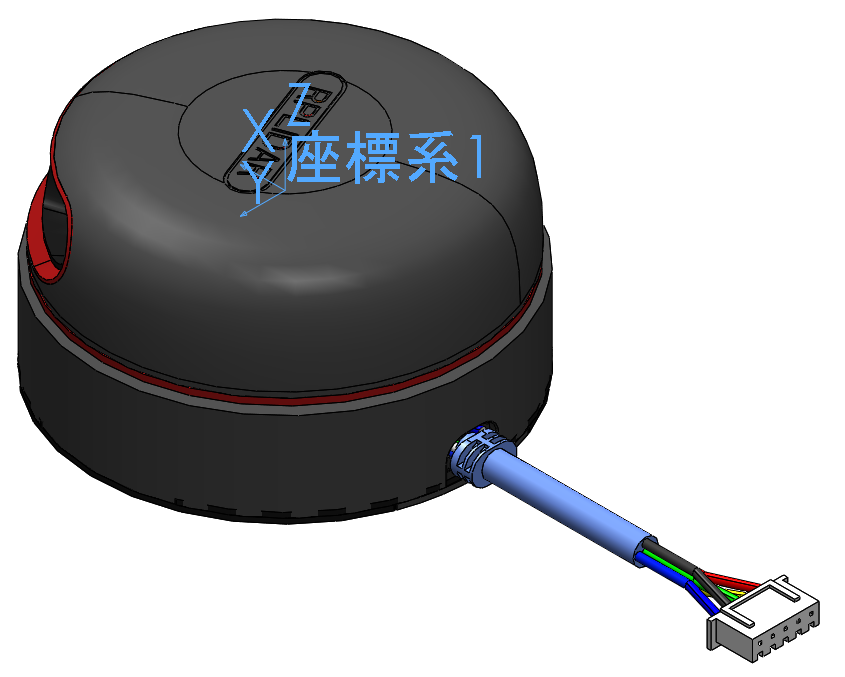
\includegraphics[height=40truemm]{images/lidar_link_coordinate.png}
  \label{fig:lidar_link_coordinate}
  \caption{Output Coordinate System of RPLiDAR Model}
\end{figure}

\subsection{\textsf{lidar.xacro}の記述}

以上を踏まえて,\textsf{lidar.xacro}を記述します.
\textsf{urdf/}ディレクトリ以下に\textsf{lidar/}ディレクトリを作り,その中にコード\ref{code:lidar_xacro}の内容を記述したファイル\textsf{lidar.xacro}を作成します.

\begin{lstlisting}[language=XML, label=code:lidar_xacro, caption=\textsf{lidar.xacro}]
<?xml version="1.0"?>
<robot xmlns:xacro="http://ros.org/wiki/xacro">
  <xacro:macro name="lidar" params="parent visual_yaw_orientation *joint_origin">
    <joint name="lidar_joint" type="fixed">
      <xacro:insert_block name="joint_origin"/>
      <parent link="${parent}"/>
      <child link="lidar_link"/>
    </joint>

    <link name="lidar_link">
      <visual>
        <origin xyz="0.0 0.0 0.0" rpy="0 0 ${visual_yaw_orientation}"/>
        <geometry>
          <mesh filename="package://adamr2_description/meshes/lidar_link.STL"/>
        </geometry>
        <material name="blue">
          <color rgba="0.0 0.0 1.0 1.0"/>
        </material>
      </visual>
    </link>
  </xacro:macro>
</robot>
\end{lstlisting}

\textsf{lidar}マクロは引数として親リンクの名前,モデルの見た目の向き,そしてジョイントの原点座標のブロックを取ります.
ジョイント原点座標とともにモデルの向きを取ることによって,RPLiDAR特有の座標系に起因する問題を解決しています.

\subsection{ルートファイルからインクルードする}

\textsf{lidar\_link}をロボットモデルに取り込みましょう.
コード\ref{code:robot_xacro_add_lidar_link}のように\textsf{robot.xacro}を編集します.
\textsf{lidar}マクロの引数\textsf{visual\_yaw\_orientation}に,\textsf{radians}マクロを使って弧度法で角度を渡しています.

\begin{lstlisting}[language=XML, label=code:robot_xacro_add_lidar_link, caption=Add \textsf{lidar\_link} to Robot Model]
<?xml version="1.0"?>
<robot name="adamr2" xmlns:xacro="http://ros.org/wiki/xacro">
  <xacro:include filename="$(find adamr2_description)/urdf/base/base.xacro"/>
  <xacro:include filename="$(find adamr2_description)/urdf/caster/caster.xacro"/>
  <xacro:include filename="$(find adamr2_description)/urdf/lidar/lidar.xacro"/>

  <!-- base_footprint -->
  <link name="base_footprint"/>

  <!-- base_link -->
  <xacro:base parent="base_footprint">
    <origin xyz="0.0 0.0 0.262"/>
  </xacro:base>

  <!-- front caster -->
  <xacro:caster prefix="back" parent="base_link">
    <origin xyz="-0.275 0.0 -0.1498"/>
  </xacro:caster>

  <!-- back caster -->
  <xacro:caster prefix="front" parent="base_link">
    <origin xyz="0.275 0.0 -0.1498" rpy="0 0 ${radians(180)}"/>
  </xacro:caster>

  <!-- lidar -->
  <xacro:lidar parent="base_link" visual_yaw_orientation="${radians(180)}">
    <origin xyz="0.275 0 0.177" rpy="0 0 ${radians(180)}"/>
  </xacro:lidar>
</robot>
\end{lstlisting}

\subsection{\textsf{rviz}による可視化}

センサを取り付けたので,\textsf{rviz}で可視化して,正しい位置に取り付けられているかどうか確認します.
\ref{sec:base_link_visualize_by_rviz}を参考に,URDFモデルを\textsf{rviz}で可視化します.

とはいえ,可視化の度に\textsf{RobotModel}を追加して,基準フレームを\textsf{base\_footprint}にして...という作業を繰り返すのは面倒です.
そこで,\textsf{rviz}の設定ファイルを保存しておいて,可視化の度に読み込むようにしてみましょう.
\textsf{rviz}を起動し,ロボットモデルの可視化が正しくできている状態(\textsf{RobotModel}を追加して\textsf{base\_footprint}を基準フレームに設定している状態)にします.
図\ref{fig:rviz_save_config_as}のように,画面左上のツールバーから「File」->「Save Config As」を選択します.

\begin{figure}[ht]
  \centering
  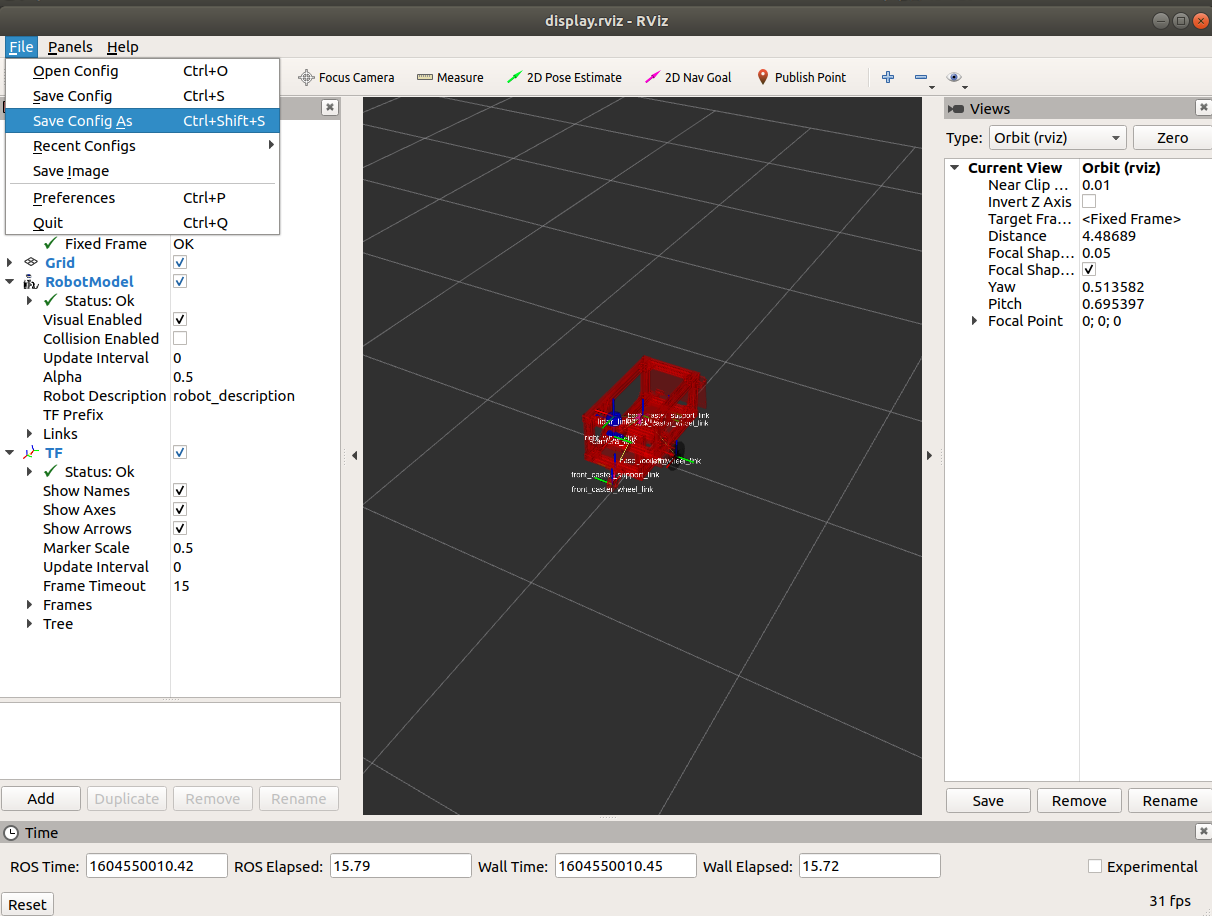
\includegraphics[height=40truemm]{images/rviz_save_config_as.png}
  \label{fig:rviz_save_config_as}
  \caption{Save \textsf{rviz} Config File}
\end{figure}

\noindent
\textsf{adamr2\_description}パッケージの中に設定ファイルを保存します.
保存場所はどこでもいいですが,わかりやすいように\textsf{rviz/}という名前のディレクトリを作り,\textsf{display.rviz}という名前で保存しましょう.

この設定ファイルを\textsf{rviz}起動時に読み込ませることで,保存しておいた設定を復元することができます.
\textsf{rviz}に設定ファイルを渡して起動するには,launchファイルを少し編集する必要があります.
コード\ref{code:rviz_load_config_at_startup}のように\textsf{display.launch}ファイルを編集します.

\begin{lstlisting}[language=XML, label=code:rviz_load_config_at_startup, caption=\textsf{rviz} Load Config File at Startup]
<launch>
  <arg name="model" default="$(find adamr2_description)/urdf/robot.xacro"/>
  <arg name="rvizconfig" default="$(find adamr2_description)/rviz/display.rviz"/>

  <param name="robot_description" command="$(find xacro)/xacro $(arg model)" />

  <node name="robot_state_publisher" pkg="robot_state_publisher" type="robot_state_publisher"/>
  <node name="rviz" pkg="rviz" type="rviz" args="-d $(arg rvizconfig)"/>
</launch>
\end{lstlisting}

launchファイルの\textsf{arg}タグを追加して,新しい変数\textsf{rvizconfig}を定義しています.
これは先程保存した\textsf{rviz}の設定ファイルへのパスです.
そして,\textsf{rviz}を起動する\textsf{node}タグの\textsf{arg}属性に設定ファイルを読み込ませるオプションを追加しています.

このlaunchファイルを実行することで,適切な設定がなされた状態でモデルが表示されます.
このように\textsf{rviz}の設定ファイルを保存しておき,実行時に読み込ませることで,作業を効率よく進めることができます.
テクニックとして覚えておいて損はないでしょう.

\textsf{lidar\_link}を追加した段階でのロボットの見た目は図\ref{fig:lidar_link_visualization}のようになります.
RPLiDARが正しい位置・向きに取り付けられていることがわかります.
リンクの座標軸が表示されていますが,これは\textsf{TF}を表示させているからです.
「Add」ボタンから追加することができます.

\begin{figure}[ht]
  \centering
  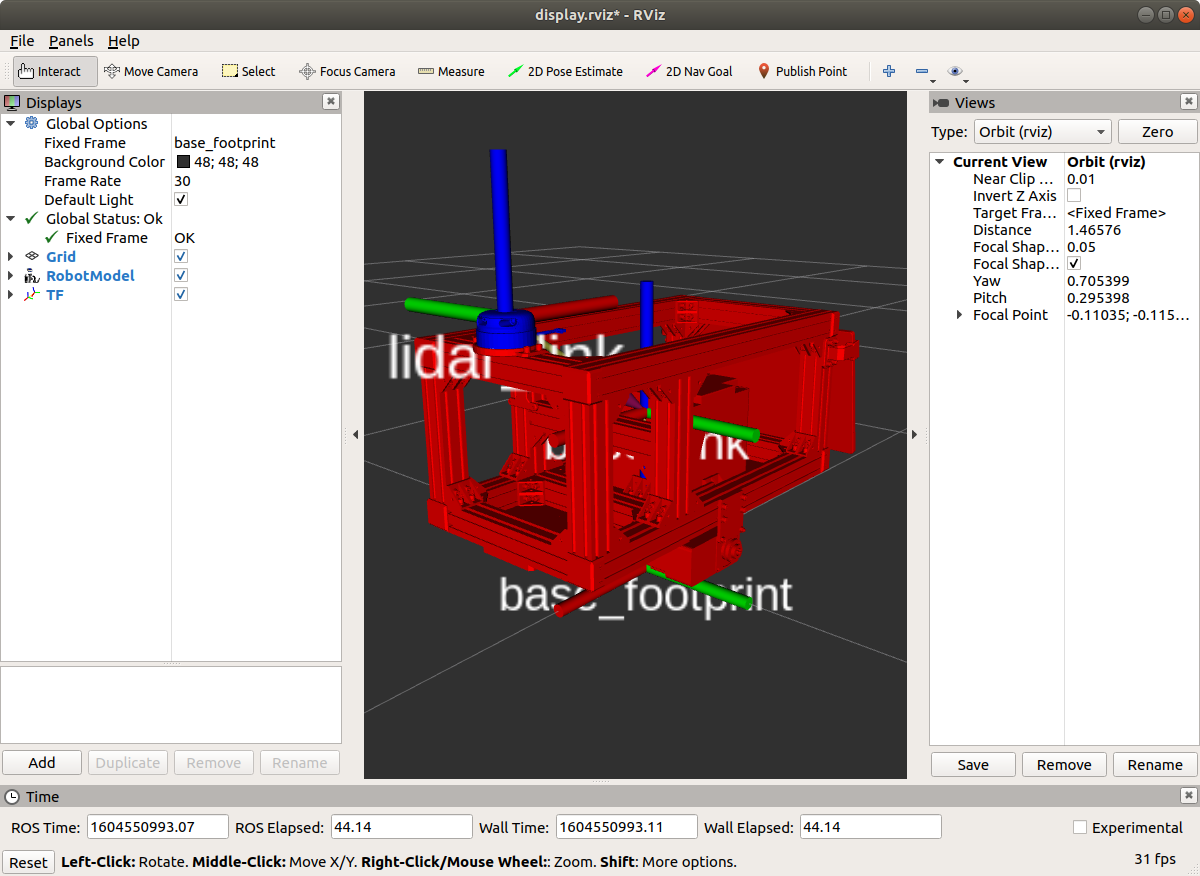
\includegraphics[height=50truemm]{images/lidar_link_visualization.png}
  \label{fig:lidar_link_visualization}
  \caption{Screenshot of \textsf{rviz}}
\end{figure}

\end{document}